\documentclass[a4paper]{article}

\usepackage{amsmath}
\usepackage{hyperref}

\usepackage{graphicx}
\usepackage{listings}
\usepackage{color}
 
\definecolor{codegreen}{rgb}{0,0.6,0}
\definecolor{codegray}{rgb}{0.5,0.5,0.5}
\definecolor{codepurple}{rgb}{0.58,0,0.82}
\definecolor{backcolour}{rgb}{0.95,0.95,0.92}
 
\lstdefinestyle{mystyle}{
    backgroundcolor=\color{backcolour},   
    commentstyle=\color{codegreen},
    keywordstyle=\color{magenta},
    numberstyle=\tiny\color{codegray},
    stringstyle=\color{codepurple},
    basicstyle=\footnotesize,
    breakatwhitespace=false,         
    breaklines=true,                 
    captionpos=b,                    
    keepspaces=true,                 
    numbers=left,                    
    numbersep=5pt,                  
    showspaces=false,                
    showstringspaces=false,
    showtabs=false,                  
    tabsize=2
}
 
\lstset{style=mystyle}


\title{Assignment 2: Linear Predictive Analysis}
\author{Pranav Sankhe| 150070009}
\date{\today}

\begin{document}

\maketitle

\section{Question}
LP re-synthesis: This is a direct continuation of Comp Assn 2. We analysed the natural speech sounds \textbackslash a\textbackslash, \textbackslash n\textbackslash, \textbackslash I\textbackslash, \textbackslash s\textbackslash. Using a suitable set of parameter estimates for each sound as obtained there, we wish to reconstruct each of the sounds. That is, use the best estimated LP filter with an ideal impulse train of the estimated pitch period as source excitation (for the voiced sounds). Carry out de-emphasis on the output waveform. For the unvoiced sound, use a white noise signal as source excitation. Set the duration of the synthesized sound to be $300$ ms at $8$ kHz sampling frequency (use $16$ kHz for the \textbackslash s\textbackslash), and view/listen to your created sound. Comment on the similarity with the original sound. What would be a good application for this analysis \& synthesis system?

\subsection{Answer}
\textbf{Comments:} \\ 
Since here, we have generated the sound pieces, using handful of the estimated parameters, this serves as an data compression technique where you can store and re-create the individual sounds very few parameters which otherwise is presented in redundant format occupying large memories. One of the plausible application of this technique is Telephone Comminication. \\
Having heard the audio of the generated sounds, except \textbackslash I\textbackslash, all others sounded convincing to me. While \textbackslash I\textbackslash being a vowel, this appeared rather unconventional to me. The ambuiguity can be attributed to the very peculiar structure of the vowel \textbackslash I\textbackslash.  


\begin{figure}[h!]
    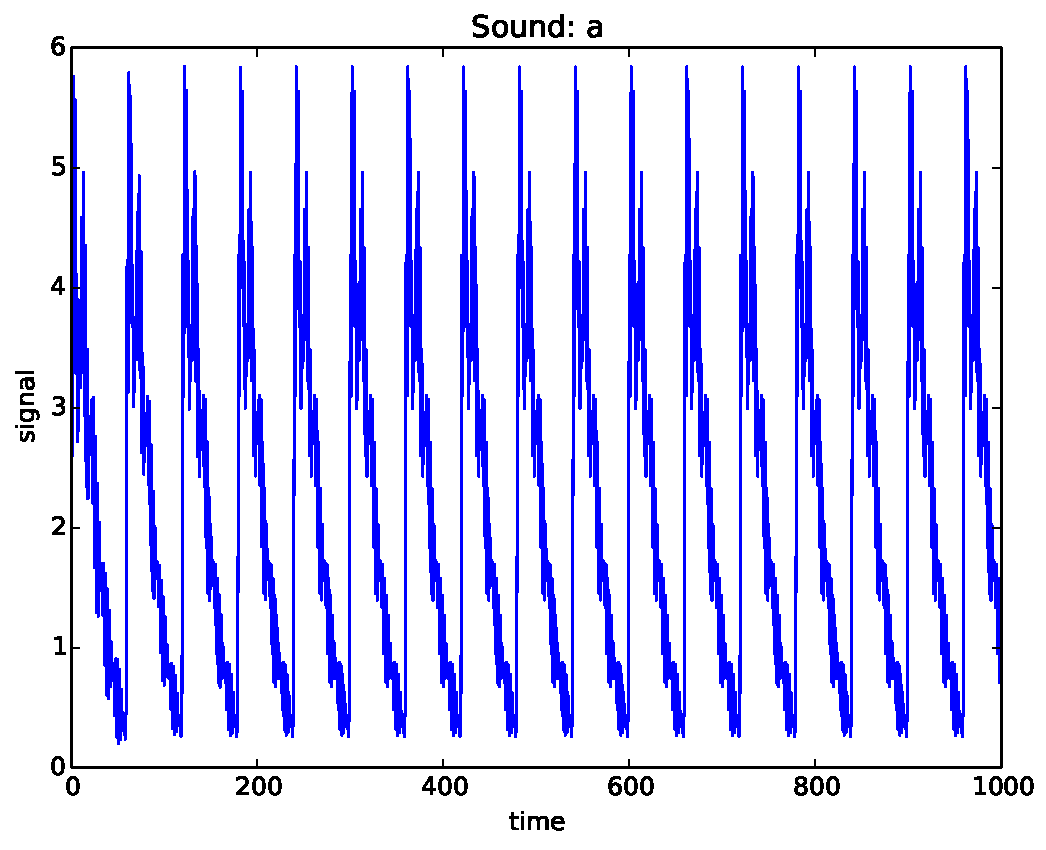
\includegraphics[width=\linewidth]{./images/q1_a.pdf}
    \caption{Reconstructed \textbackslash a\textbackslash}
    \label{fig:1}
\end{figure}

\begin{figure}[h!]
    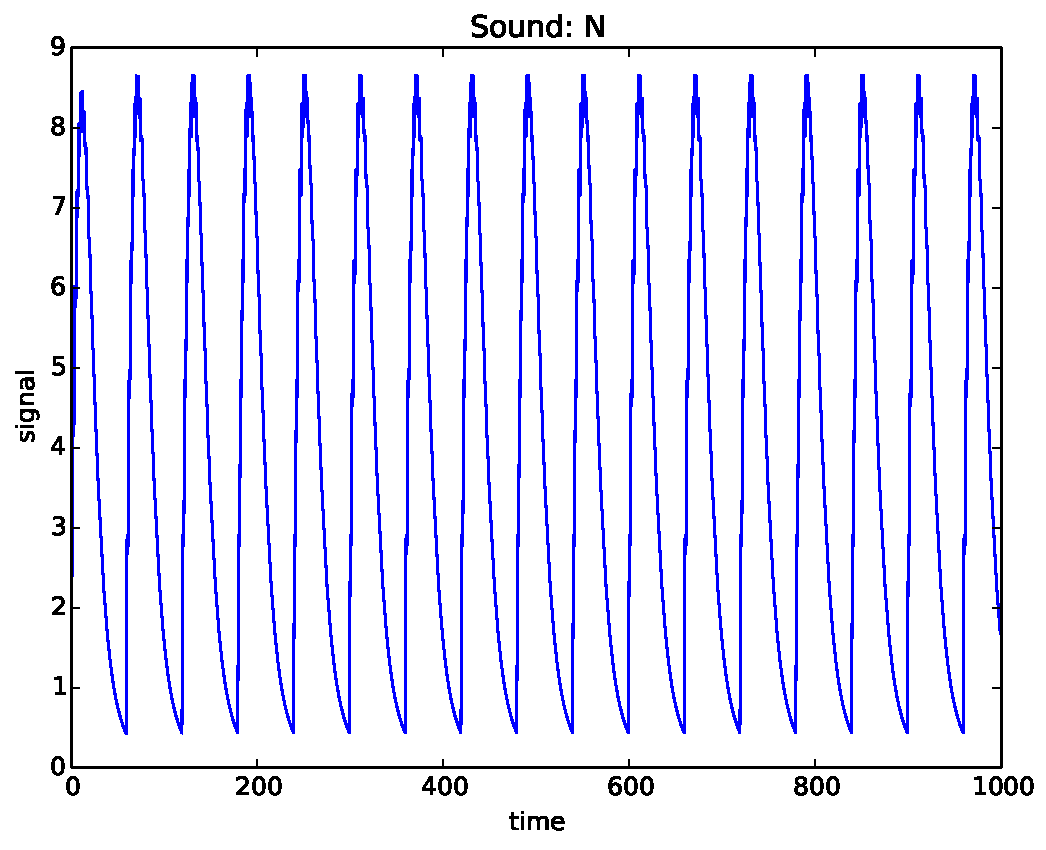
\includegraphics[width=\linewidth]{./images/q1_n.pdf}
    \caption{Reconstructed \textbackslash n\textbackslash}
    \label{fig:1}
\end{figure}

\begin{figure}[h!]
    \includegraphics[width=\linewidth]{./images/q1_I.pdf}
    \caption{Reconstructed \textbackslash I\textbackslash}
    \label{fig:1}
\end{figure}

\begin{figure}[h!]
    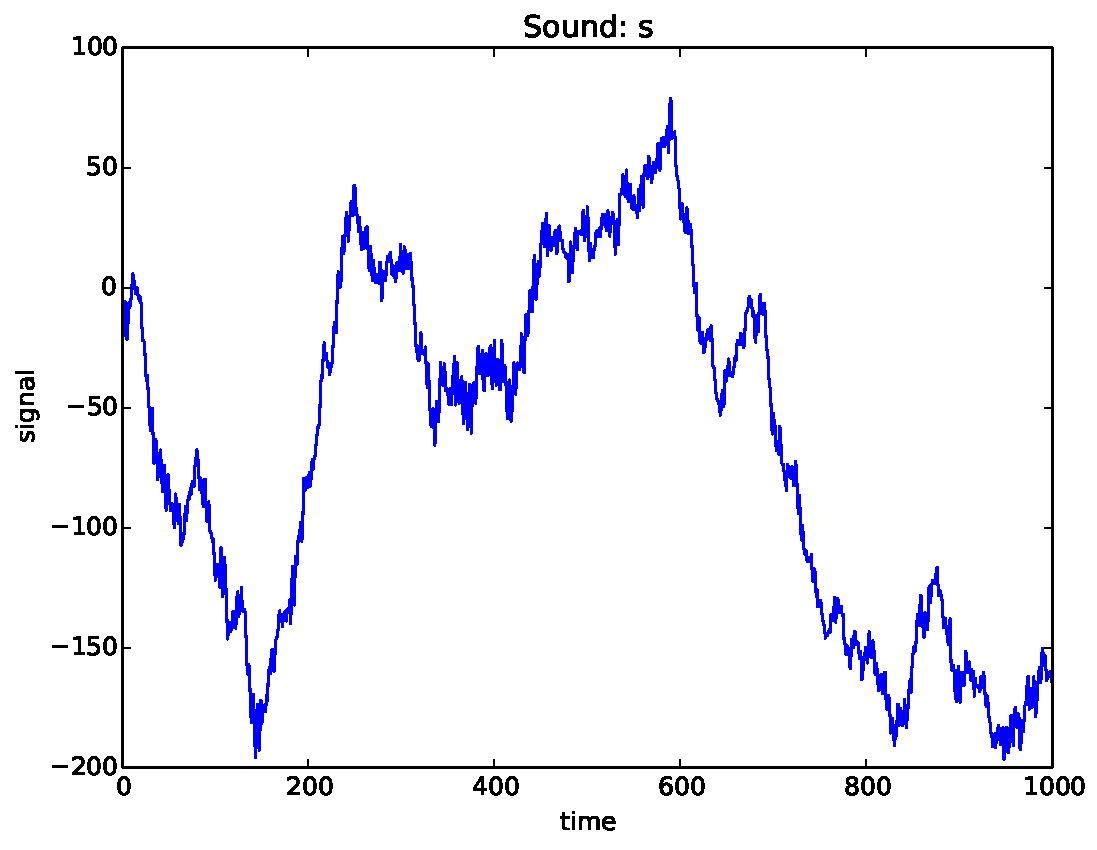
\includegraphics[width=\linewidth]{./images/q1_s.pdf}
    \caption{Reconstructed \textbackslash s\textbackslash}
    \label{fig:1}
\end{figure}




File containing all the paramaters:
\begin{lstlisting}[language=Python, caption=params.py]
F0 = 8000.0/60.0
sounds = ['a', 'N', 'I' , 's'] 
samp_freq = 8000.0
duration  = 300.0/1000.0

a_den  = [ 1.0, 0.30770776, -0.70935154, -0.01249522, 0.15924091, 0.03700667, 0.15999816, -0.03421146, -0.09653191, -0.25471351, -0.03752092]
a_num = [4.13339752, 0.0, 0.0, 0.0, 0.0, 0.0, 0.0, 0.0, 0.0, 0.0, 0.0]

n_den = [1.0, -2.18439905e-02, -8.92734898e-01, 4.32920514e-04, 4.89812545e-04, 4.89186592e-04, 4.88165983e-04, 4.86755417e-04, 4.86350841e-04, 2.22938139e-02, 6.37348443e-02]
n_num = [2.49895716, 0.0, 0.0, 0.0, 0.0, 0.0, 0.0, 0.0, 0.0, 0.0, 0.0]

i_den = [1.0, -4.30221491e-02, -8.82316432e-01, -2.98545924e-04, 4.46520736e-04, 4.46443384e-04, 4.45346265e-04, 4.44658817e-04, 1.39040245e-03, 9.07980247e-02, -1.67148707e-02]
i_num = [2.39543144, 0.0, 0.0, 0.0, 0.0, 0.0, 0.0, 0.0, 0.0, 0.0, 0.0]

s_den = [1., -0.014787, 0.26017104, -0.27388149, -0.3356718, -0.16531149, -0.04300548, 0.17950459, -0.03551942, -0.08449707, -0.05001272, -0.08581098, 0.0386388, -0.10588742, 0.01688407, -0.04029857, -0.00275163, -0.05118139, -0.13576579, -0.03593119, -0.0137991]
s_num = [5.29962619, 0.0, 0.0, 0.0, 0.0, 0.0, 0.0, 0.0, 0.0, 0.0, 0.0, 0.0, 0.0, 0.0, 0.0, 0.0, 0.0, 0.0, 0.0, 0.0, 0.0]
\end{lstlisting}

main file: 
\begin{lstlisting}[language=Python, caption=q1.py]
from scipy import signal
import numpy as np
import matplotlib.pyplot as plt
from scipy.io import wavfile
import params

F0 = params.F0
sounds = params.sounds

a_den = params.a_den
n_den = params.n_den
i_den = params.i_den
s_den = params.s_den
den = [a_den, n_den, i_den, s_den]

a_num = params.a_num
n_num = params.n_num
i_num = params.i_num
s_num = params.s_num
num = [a_num, n_num, i_num, s_num]

for i in range(len(sounds)):
    
    duration = params.duration
    samp_freq = params.samp_freq
    t = np.linspace(0, duration, duration*samp_freq, endpoint=False)
    sig = (1 + signal.square(2 * np.pi * F0 * t, duty=0.01))/2
    if i == 3:
        samp_freq = samp_freq*2
        sig = np.random.normal(0, 1, int(duration*samp_freq))

    
    result = signal.lfilter(num[i], den[i], sig)
    
    result = signal.lfilter(np.asarray([1.0, 0.0]), np.asarray([1, -15.0/16.0]), result)
    fig = plt.figure()
    plt.plot(result[0:1000])
    plt.title("Sound: " + sounds[i])
    plt.xlabel('time')
    plt.ylabel('signal')
    fig.savefig("Sound: " + sounds[i] + ".pdf", bbox_inches='tight')
    wavfile.write(sounds[i] + '.wav', samp_freq, np.int16(result/np.max(result)*32767))
\end{lstlisting}

\section{Question}
Next, consider the synthetic signal (for \textbackslash a\textbackslash) reconstructed from LP coefficients ($p=10$) and pulse train in part $1$. Compute the real cepstrum and obtain the spectral envelope (dB) via cepstral liftering. Compare this estimated spectral envelope with the true LP magnitude spectrum. Observe and comment on the changes in cepstral estimate with different duration lifters.

\subsection{Answer}
\textbf{Comments:} \\ 
The window length might be chosen to give sufficient frequency resolution, however, due to the time-space resolution trade-off of FFT analysis, the resulting time resolution may not be adequate, and thus miss fast audio transients not being centered or isolated in one window
As we can see in the plots, with extremely less window length, the windowed signal itself converges towards an envelope. 
But from the plots we can see that as we increase the window length the peaks in the spectrum get well captured by the cepstrum envelope. 
However, reducinng the analysis window duration has little effect on distant harmonic energy leakage on the spectral valleys around a local harmonic. 

\begin{figure}[h!]
    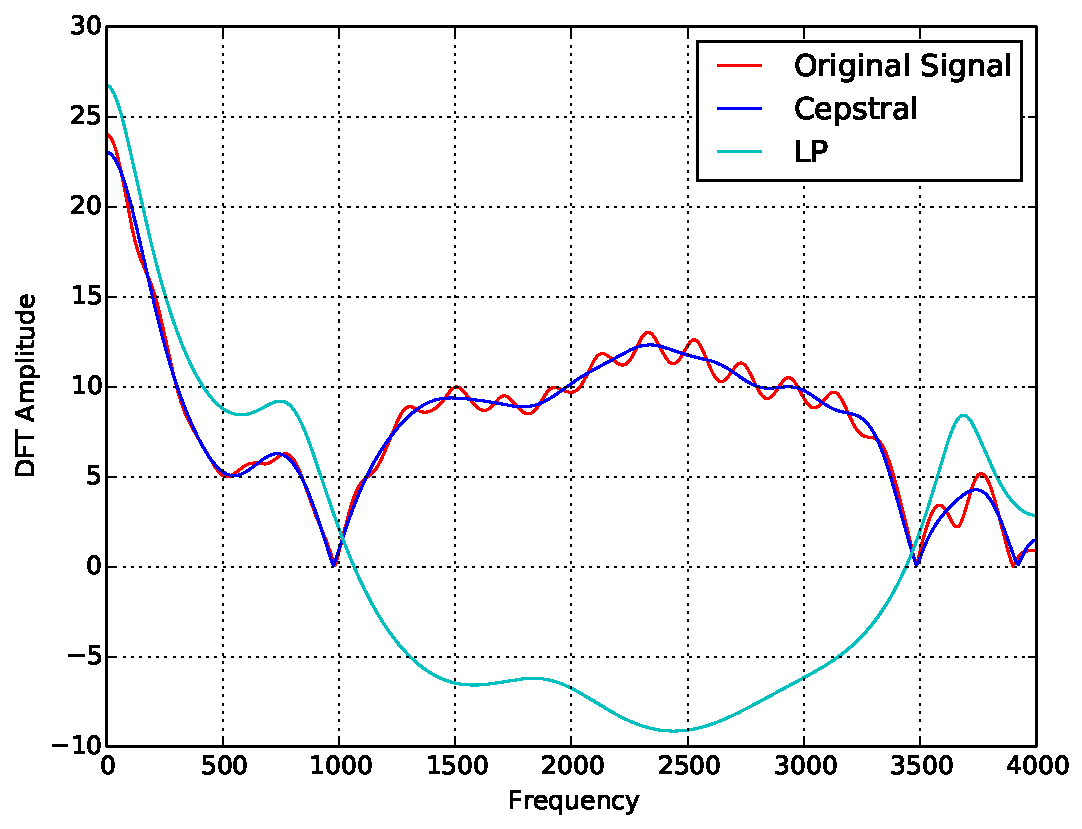
\includegraphics[width=\linewidth]{./images/a_winlen=10.pdf}
    \caption{Cepstrum Envelope for \textbackslash a\textbackslash with $window_duration=10 ms$}
    \label{fig:1}
\end{figure}

\begin{figure}[h!]
    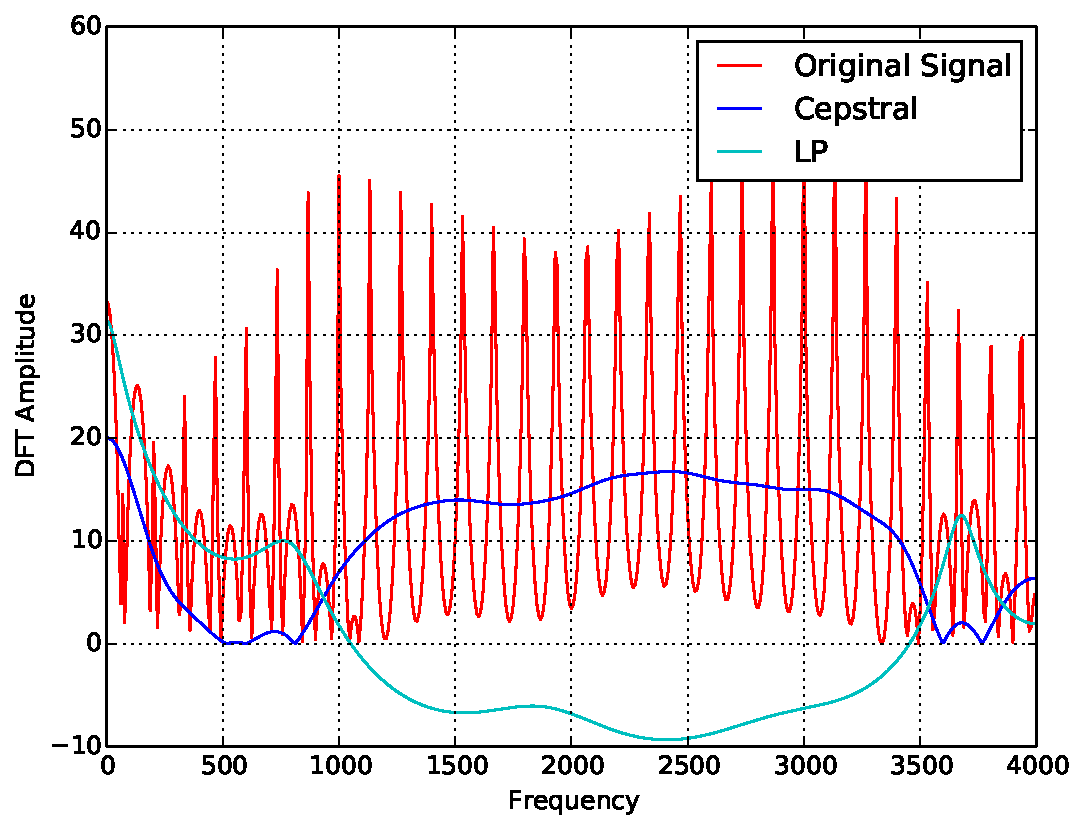
\includegraphics[width=\linewidth]{./images/a_winlen=30.pdf}
    \caption{Cepstrum Envelope for \textbackslash a\textbackslash with $window_duration=30 ms$}
    \label{fig:1}
\end{figure}

\begin{figure}[h!]
    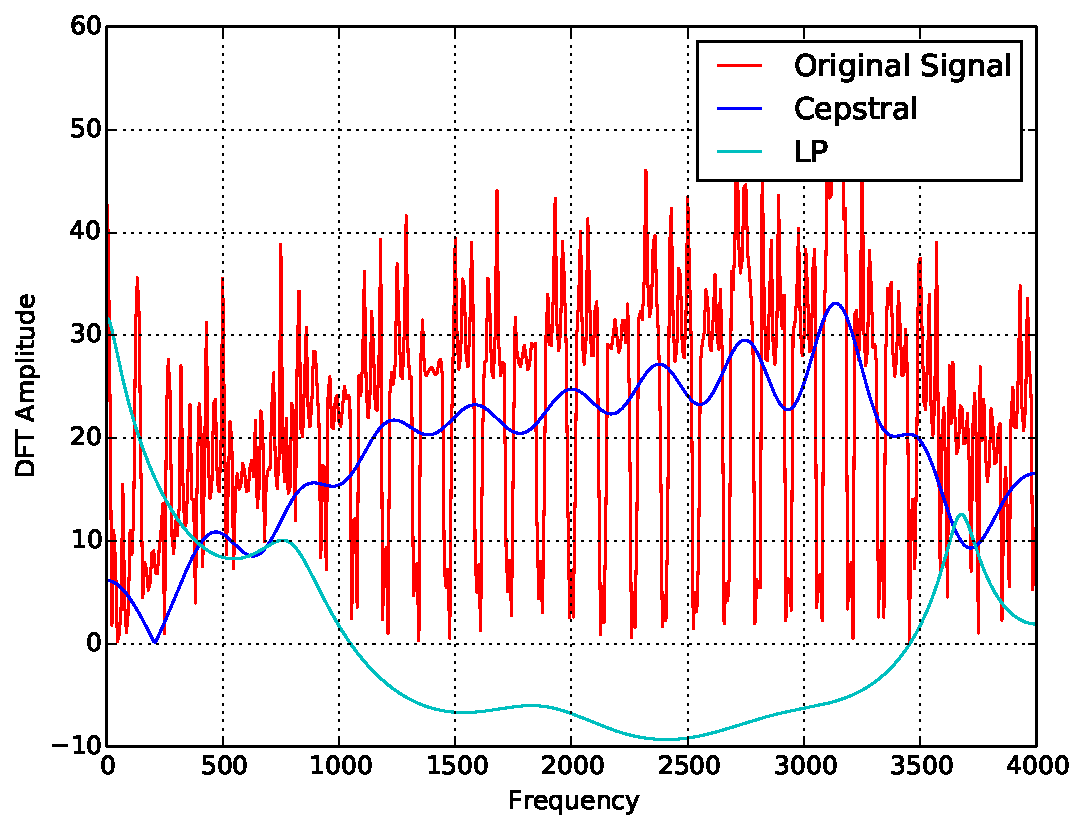
\includegraphics[width=\linewidth]{./images/a_winlen=100.pdf}
    \caption{Cepstrum Envelope for \textbackslash a\textbackslash with $window_duration=100 ms$}
    \label{fig:1}
\end{figure}

\begin{lstlisting}[language=Python, caption=params.py]
F0 = 8000.0/60.0
sounds = ['a', 'N', 'I' , 's'] 
samp_freq = 8000.0
duration  = 300.0/1000.0

a_den  = [ 1.0, 0.30770776, -0.70935154, -0.01249522, 0.15924091, 0.03700667, 0.15999816, -0.03421146, -0.09653191, -0.25471351, -0.03752092]
a_num = [4.13339752, 0.0, 0.0, 0.0, 0.0, 0.0, 0.0, 0.0, 0.0, 0.0, 0.0]

n_den = [1.0, -2.18439905e-02, -8.92734898e-01, 4.32920514e-04, 4.89812545e-04, 4.89186592e-04, 4.88165983e-04, 4.86755417e-04, 4.86350841e-04, 2.22938139e-02, 6.37348443e-02]
n_num = [2.49895716, 0.0, 0.0, 0.0, 0.0, 0.0, 0.0, 0.0, 0.0, 0.0, 0.0]

i_den = [1.0, -4.30221491e-02, -8.82316432e-01, -2.98545924e-04, 4.46520736e-04, 4.46443384e-04, 4.45346265e-04, 4.44658817e-04, 1.39040245e-03, 9.07980247e-02, -1.67148707e-02]
i_num = [2.39543144, 0.0, 0.0, 0.0, 0.0, 0.0, 0.0, 0.0, 0.0, 0.0, 0.0]

s_den = [1., -0.014787, 0.26017104, -0.27388149, -0.3356718, -0.16531149, -0.04300548, 0.17950459, -0.03551942, -0.08449707, -0.05001272, -0.08581098, 0.0386388, -0.10588742, 0.01688407, -0.04029857, -0.00275163, -0.05118139, -0.13576579, -0.03593119, -0.0137991]
s_num = [5.29962619, 0.0, 0.0, 0.0, 0.0, 0.0, 0.0, 0.0, 0.0, 0.0, 0.0, 0.0, 0.0, 0.0, 0.0, 0.0, 0.0, 0.0, 0.0, 0.0, 0.0]
\end{lstlisting}


File containing all the paramaters:
\begin{lstlisting}[language=Python, caption=params.py]
filename = 'a.wav'
window_duration = 10.0/1000.0
fft_length = 1024
order = 10
N_cep = 25
\end{lstlisting}

main file: 
\begin{lstlisting}[language=Python, caption=q2.py]
from scipy import signal
import numpy as np
from math import pi
import matplotlib.pyplot as plt
from scipy.io import wavfile
import params

def autocorr(x):
    result = np.correlate(x, x, mode='full')
    return result[int(result.size/2):]


[sample_rate, y] = wavfile.read('a.wav');
y = y/32768.0
window_duration = params.window_duration 
num_samples = sample_rate*window_duration
fft_length = params.fft_length
fig = plt.figure()

window = y[int((len(y) - num_samples)/2):int((len(y) + num_samples)/2)]*np.hamming(num_samples)


log_fft = np.log10(np.abs(np.fft.fft(window, fft_length)))
cepstrum = np.real(np.fft.ifft(log_fft))


N_cep = params.N_cep
cepstrum[N_cep:(cepstrum.shape[-1]-N_cep)] = 0

# Take the DFT and plot it
cepstrum_dft = np.abs(np.fft.fft(cepstrum, fft_length))
freq = np.fft.fftfreq(cepstrum_dft.shape[-1], 1/float(sample_rate))

plt.plot(freq[:len(freq)/2], 20*np.abs(log_fft[:len(log_fft)/2]), 'r')
plt.plot(freq[:len(freq)/2], 20*np.abs(cepstrum_dft[:len(cepstrum_dft)/2]), 'b')



order = params.order

R = autocorr(window)
error = np.zeros(order+1)
error[0] = R[0]
G = np.zeros(order + 1)

coeffs = np.zeros(order+1)
dummy_coeffs = np.zeros(order + 1)


for i in range(1, order +1):
    reflec_coeffs = 0
    dummy_coeffs[1:len(coeffs)] = coeffs[1:len(coeffs)]
    
    for j in range(1, i):
        reflec_coeffs = reflec_coeffs + dummy_coeffs[j]*R[i-j]
    reflec_coeffs = (R[i] - reflec_coeffs)/error[i-1]

    coeffs[i] = reflec_coeffs

    for j in range(1, i):
        coeffs[j] = dummy_coeffs[j] - reflec_coeffs*dummy_coeffs[i-j]

    error[i] = (1-np.square(reflec_coeffs))*error[i-1]

coeffs[0] = 1.0
coeffs[1:len(coeffs)] = -coeffs[1:len(coeffs)]
num_coeffs = np.zeros(coeffs.shape)
num_coeffs[0] = 1
G[i] = np.sqrt(error[i])
w, h = signal.freqz(num_coeffs, coeffs)

plt.plot(sample_rate*w/(2*pi), 20 * np.log10(abs(h)), 'c')
plt.ylabel('DFT Amplitude')
plt.xlabel('Frequency')
plt.legend(['Original Signal', 'Cepstral', 'LP'])
plt.grid()
fig.savefig('a_winlen=' + str(window_duration*1000) +  ".pdf", bbox_inches='tight')

plt.show()
\end{lstlisting}





\section{Question}
Finally, we wish to carry out the cepstral analyses of the same natural speech sounds. Obtain the real cepstrum from a 30 ms segment for each of the phones (of the natural speech as in part 1). Estimate the voicing and pitch of the segment from the real cepstrum. Use cepstral filtering to obtain the spectral envelope (dB) in each case. Compare it with the corresponding LP (p=10) magnitude spectrum obtained previously by superposing both on the actual magnitude spectrum of the windowed signal. (Obtain the vocal tract magnitude response of /s/ sampled at 16 kHz using LP order = 18.)


\subsection{Answer}

\begin{figure}[h!]
    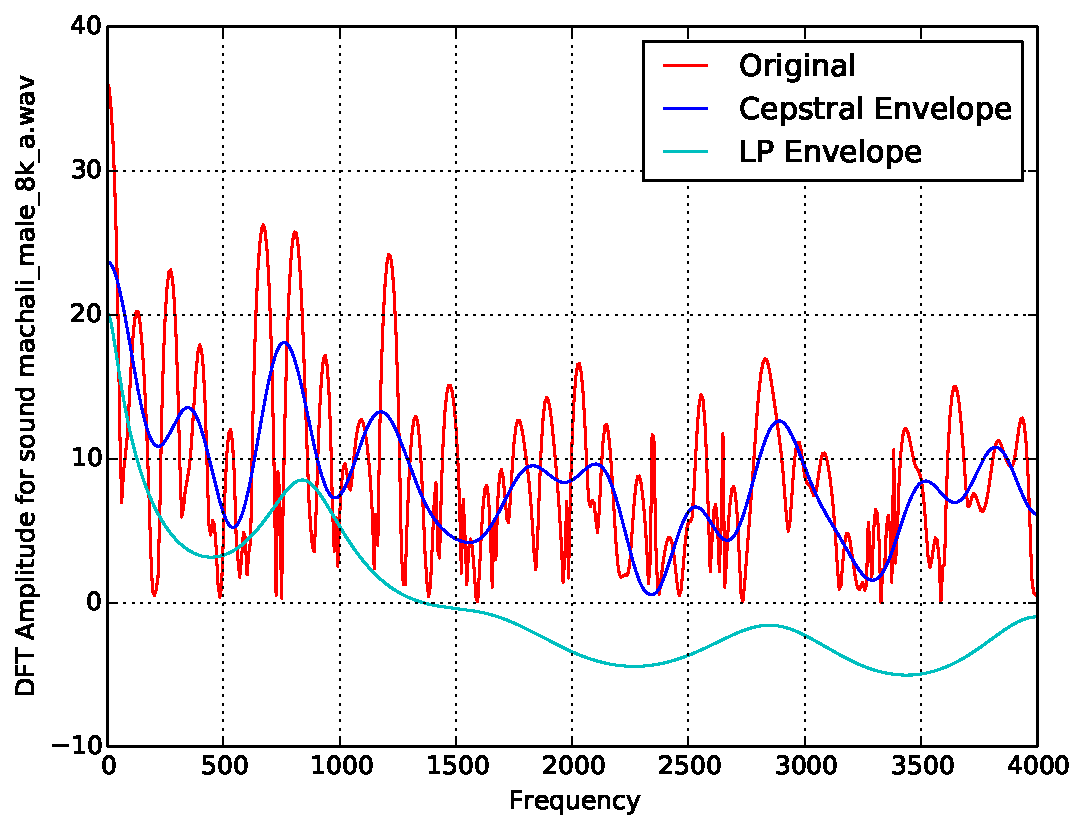
\includegraphics[width=\linewidth]{./images/q3machali_male_8k_a.pdf}
    \caption{Sound \textbackslash a\textbackslash in \textit{machali}}
    \label{fig:1}
\end{figure}

\begin{figure}[h!]
    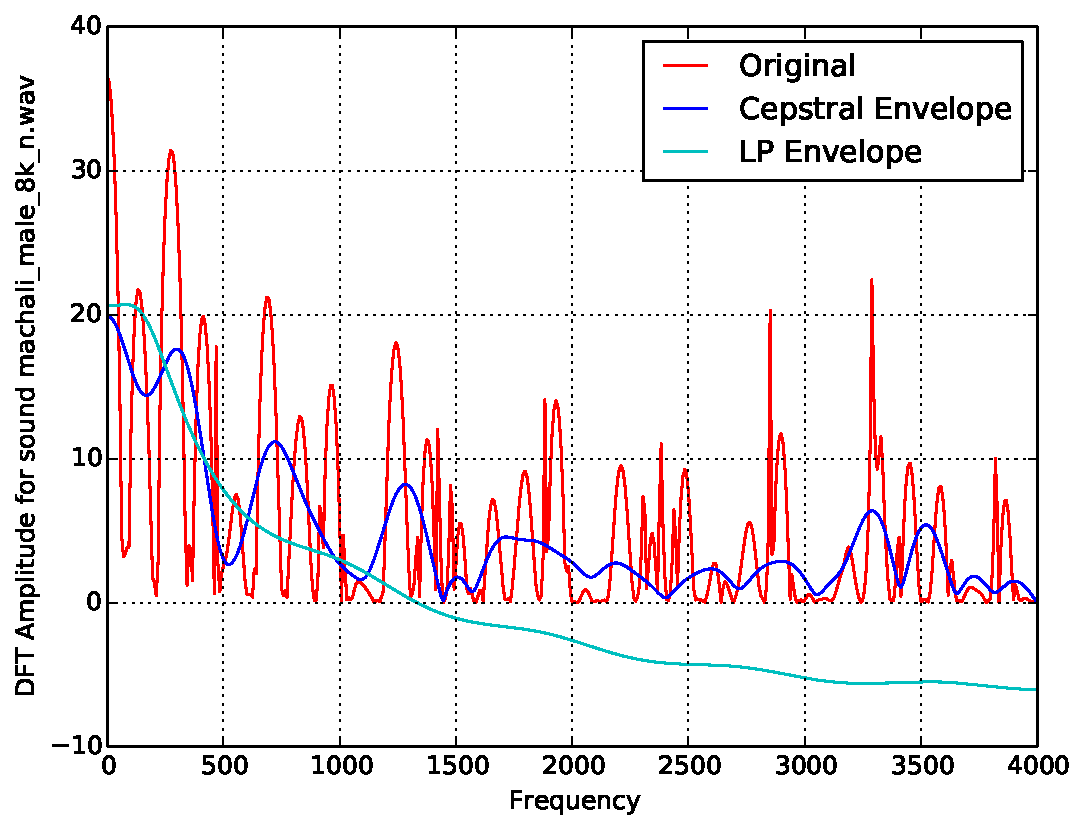
\includegraphics[width=\linewidth]{./images/q3machali_male_8k_n.pdf}
    \caption{Sound \textbackslash n\textbackslash in \textit{machali}}
    \label{fig:1}
\end{figure}

\begin{figure}[h!]
    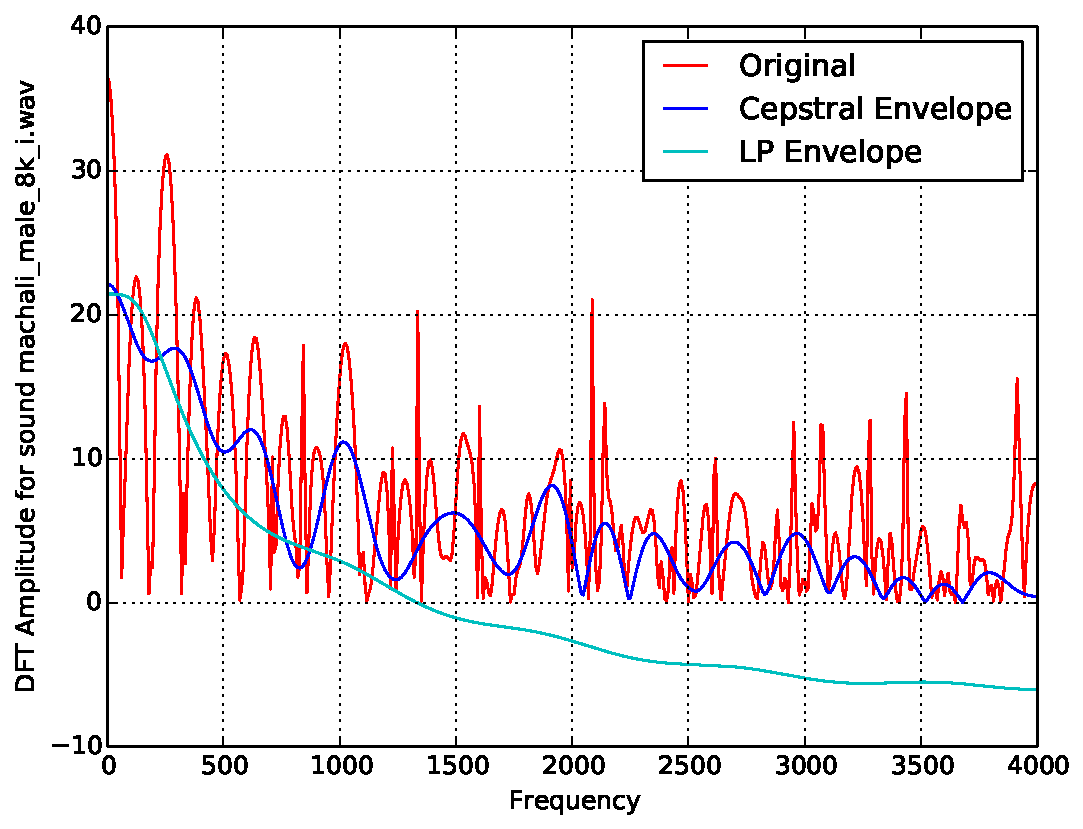
\includegraphics[width=\linewidth]{./images/q3machali_male_8k_i.pdf}
    \caption{Sound \textbackslash I\textbackslash in \textit{machali}}
    \label{fig:1}
\end{figure}

\begin{figure}[h!]
    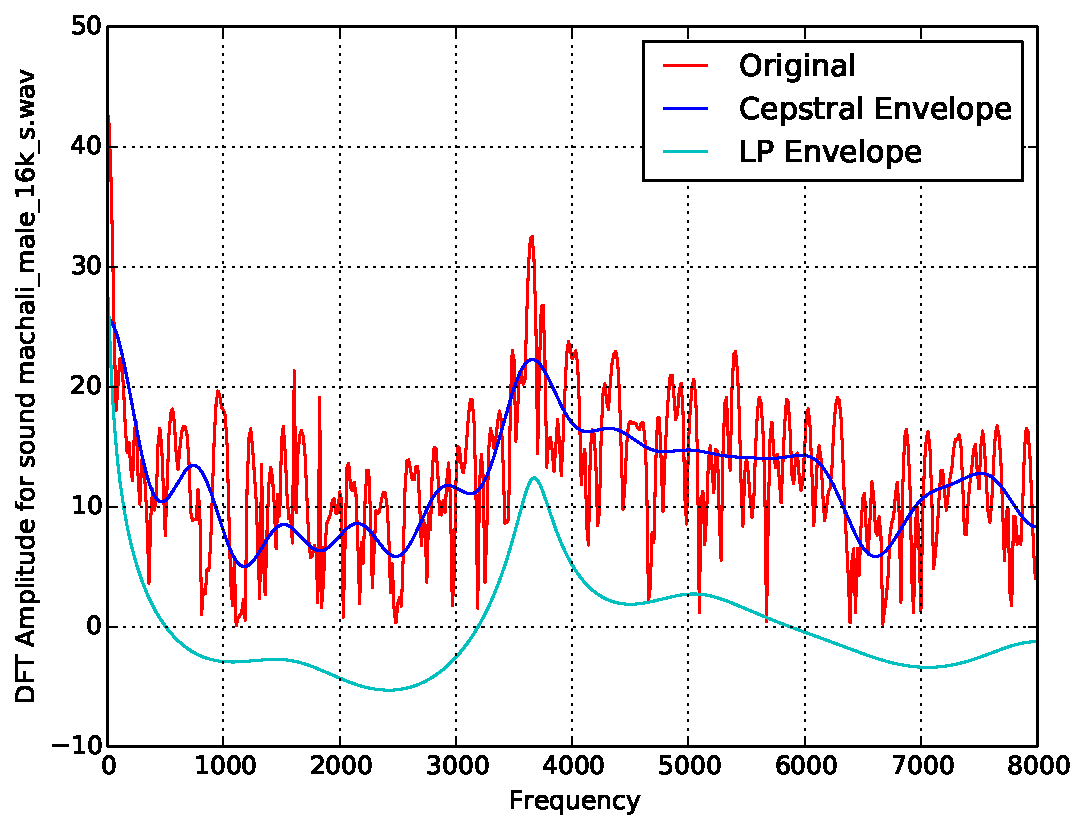
\includegraphics[width=\linewidth]{./images/q3machali_male_16k_s.pdf}
    \caption{Sound \textbackslash s\textbackslash in \textit{machali}}
    \label{fig:1}
\end{figure}



\begin{lstlisting}[language=Python, caption=params.py]
filenames = ['machali_male_8k_a.wav', 'machali_male_8k_n.wav', 'machali_male_8k_i.wav', 'machali_male_16k_s.wav']
duration = 30.0/1000.0
fft_length = 1024
cep_N =  25
order = 10
\end{lstlisting}

main file: 
\begin{lstlisting}[language=Python, caption=q2.py]
from scipy import signal
import numpy as np
from math import pi
import matplotlib.pyplot as plt
from scipy.io import wavfile
import params

def autocorr(x):
    result = np.correlate(x, x, mode='full')
    return result[int(result.size/2):]


filenames = params.filenames
    
for filename in filenames:
    samp_rate, y = wavfile.read(filename)
    y = y/32768
    duration = params.duration
    num_samples = samp_rate*duration 
    fft_length = params.fft_length

    window = y[int((len(y) - num_samples)/2):int((len(y) + num_samples)/2)]*np.hamming(num_samples)

    log_fft = np.log10(np.abs(np.fft.fft(window, fft_length)))
    cepstrum = np.real(np.fft.ifft(log_fft))


    cep_N =  params.cep_N
    cepstrum[cep_N:(cepstrum.shape[-1]-cep_N)] = 0


    cepstrum_fft = np.abs(np.fft.fft(cepstrum, fft_length))
    freq = np.fft.fftfreq(cepstrum_fft.shape[-1], 1/float(samp_rate))
    fig = plt.figure()
    plt.plot(freq[:len(freq)/2], 20*np.abs(log_fft[:len(log_fft)/2]), 'r')
    plt.plot(freq[:len(freq)/2], 20*np.abs(cepstrum_fft[:len(cepstrum_fft)/2]), 'b')


    order = params.order 

    R = autocorr(window)
    error = np.zeros(order+1)
    error[0] = R[0]
    G = np.zeros(order + 1)

    coeffs = np.zeros(order+1)
    dummy_coeffs = np.zeros(order + 1)


    for i in range(1, order +1):
        reflec_coeffs = 0
        dummy_coeffs[1:len(coeffs)] = coeffs[1:len(coeffs)]
        
        for j in range(1, i):
            reflec_coeffs = reflec_coeffs + dummy_coeffs[j]*R[i-j]
        reflec_coeffs = (R[i] - reflec_coeffs)/error[i-1]

        coeffs[i] = reflec_coeffs

        for j in range(1, i):
            coeffs[j] = dummy_coeffs[j] - reflec_coeffs*dummy_coeffs[i-j]

        error[i] = (1-np.square(reflec_coeffs))*error[i-1]

    coeffs[0] = 1.0
    coeffs[1:len(coeffs)] = -coeffs[1:len(coeffs)]
    num_coeffs = np.zeros(coeffs.shape)
    num_coeffs[0] = 1
    G[i] = np.sqrt(error[i])
    w, h = signal.freqz(num_coeffs, coeffs)
    plt.plot(samp_rate*w/(2*pi), 20 * np.log10(abs(h)), 'c')
    plt.ylabel('DFT Amplitude for sound ' + filename)
    plt.xlabel('Frequency')
    plt.legend(['Original', 'Cepstral Envelope', 'LP Envelope'])
    plt.grid()

    fig.savefig('q3'+ filename.split('.')[0] + ".pdf", bbox_inches='tight')

plt.show()    
\end{lstlisting}





\end{document}